%!TEX root = ../main.tex

\chapter{Results}\label{cha:results}

In this chapter, the implementation of a fingerprint function within the Axelrod-Python library will be examined.
This includes the addition of two strategy transformers, the Dual and JossAnn as defined in \ref{}. %TODO
Then several results will be presented where analytical fingerprints are compared with analytical ones.
A discussion that compares different fingerprints of strategies within Axelrod-Python will also be given.

\section{The Dual}
The dual of a strategy is defined such that when when the original strategy and the dual are presented with identical histories they will return opposite actions.
This relies on knowledge of how the original strategy would have behaved in a given situation, would be impractical to infer from the source code, however, the required behaviour can be achieved by having the original strategy as an attribute of the dual.
Whenever the dual has to submit a move, it can first get the original strategy to suggest what move should it would have made, and then flip that action.

\IncMargin{1.2em}
\begin{algorithm}[H]
 \KwData{A strategy}
 \KwResult{The d of the strategy}{}
  \If{First Turn}{
   create copy of original strategy\;}
  simulate original strategy\;
  update original strategy's history/internal state\;
  \Return{Flip of original strategy's move}
 \caption{The Dual of a Strategy}
\end{algorithm}\DecMargin{1.5em}

\section{Implementation of Fingerprinting}\label{sec:fingerprint-implementation}

As defined in section a fingerprint function is merely the expected score of a strategy when played against a Joss-Ann transformer of a probe with varying parameters. %TODO reference definition
An approximation to this has been implemented within the Axelrod-Python library.
It begins by taking a sample of the $x,y$ values that may define the Joss-Ann Transformer.
The strategy then plays a match against the a transformer with each of the sampled values.
The average score per turn can be calculated at the end of each match which corresponds to the expected score required by the exact fingerprint function.
The whole process can be repeated for reliability and the resulting scores plotted.
This method has been modelled as a spatial tournament within Axelrod-Python, where the strategy plays all of the probes and a probe only plays the strategy.
For an example with 9 probes, see Figure \ref{fig:spatialtourn}.

\begin{figure}[!hbtp]
    \begin{center}
        \includestandalone{../img/spatial_tournament}
        \caption{A spatial tournament for the strategy against 9 probes}\label{fig:spatialtourn}
    \end{center}
\end{figure}


Whether the numerical fingerprint matches the analytical one relies heavily on the choice of parameters.
Specifically the \mintinline{python}{turns, repetetitons} and \mintinline{python}{step} variables.
The \mintinline{python}{step} variable determines the number of $x,y$ values taken.
Listing \ref{lst:create-points} shows how a grid of points is constructed over the unit square where the distance between each point is taken as \mintinline{python}{step}.
Therefore, a smaller \mintinline{python}{step} variable means more points are created and so greater detail is included in the plot (similar to pixels).

\begin{listing}[hbtp!]
\begin{SourceCode}
def create_points(step):
    """Creates a set of Points over the unit square.
    A Point has coordinates (x, y). This function constructs points that are
    separated by a step equal to `step`. The points are over the unit
    square which implies that the number created will be (1/`step` + 1)^2.
    Parameters
    ----------
    step : float
        The separation between each Point. Smaller steps will produce more
        Points with coordinates that will be closer together.
    Returns
    ----------
    points : list
        of Point objects with coordinates (x, y)
    """
    num = int((1 / step) // 1) + 1
    points = [Point(j, k) for j in np.linspace(0, 1, num)
              for k in np.linspace(0, 1, num)]

    return points
\end{SourceCode}
\caption{Axelrod-Python code to create a sample of $x,y$ points}
\label{lst:create-points}
\end{listing}

The \mintinline{python}{turns} variable determines how many interactions there will be in a match.
Enough turns must be selected to ensure that steady long term behaviour is reached otherwise the average score per turn can be wildly innacurate.
However, once this state is reached, extending the number of turns has a minimal effect on the accuracy of the plot.
The \mintinline{python}{repetitions} variable decides how many times the tournament would be repeated.
Fingerprinting is a random process and high repetitions helps to reduce the effects of this.

\begin{listing}[hbtp!]
\begin{SourceCode}
def fingerprint(self, turns=50, repetitions=10, step=0.01, processes=None,
                filename=None, in_memory=False, progress_bar=True):
    """Build and play the spatial tournament.

    Creates the probes and their edges then builds a spatial tournament.
    When the coordinates of the probe sum to more than 1, the dual of the
    probe is taken instead and then the Joss-Ann Transformer is applied. If
    the coordinates sum to less than 1 (or equal), then only the Joss-Ann is
    applied, a dual is not required.

    Parameters
    ----------
    turns : integer, optional
        The number of turns per match
    repetitions : integer, optional
        The number of times the round robin should be repeated
    step : float, optional
        The separation between each Point. Smaller steps will
        produce more Points that will be closer together.
    processes : integer, optional
        The number of processes to be used for parallel processing
    progress_bar : bool
        Whether or not to create a progress bar which will be updated

    Returns
    ----------
    self.data : dictionary
        A dictionary where the keys are coordinates of the form (x, y) and
        the values are the mean score for the corresponding interactions.
    """
\end{SourceCode}
\caption{Axelrod-Python docstring for the fingerprint function}
\label{lst:fingerprint-docstring}
\end{listing}


\section{Comparison of Analytical and Numerical Plots}

In figure \ref{fig:ashlock-fingerprints}, several analytical fingerprints from previous literature are shown \cite{Ashlock2004}.
Colourings and shadings are used to make certain features stand out, and an attempt to replicate this behaviour was implemented in Axelrod-Python.
The popular plotting library matplotlib has many options for different colour maps which are demonstrated in Appendix . %TODO

\begin{figure}[hbtp!]
    \begin{center}
        \includegraphics[width = 0.6\textwidth]{../img/MultipleFingerprintsAshlock}
    \end{center}
    \caption{Shaded plots of the fingerprint functions for the strategies TitForTat, Psycho, AllD and AllC, in reading order.}
    \label{fig:ashlock-fingerprints}
\end{figure}

Using the analytical fingerprints from previous literature, and the fingerprint formulae provided alongside them, the most appropriate colour map was chosen.
The colour map Seismic was selected due to its divergent properties (although all colour maps are available within the library).
With divergent colour maps, all extreme values (high or low) are coloured, whilst mid range values are left white.
This highlights areas of interest, and in Figure \ref{fig:WSLS-ashlock-comparison} it can be seen that this matches previous work very well.

\begin{figure}[hbtp!]
\centering
\subfloat[WSLS fingerprint from previous literature]{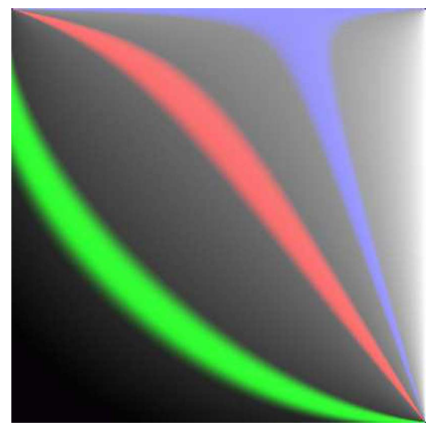
\includegraphics[width = 0.4\textwidth]{../img/WSLS-Ashlock}}
\subfloat[Analytical WSLS fingerprint demonstrating Seismic colouring]{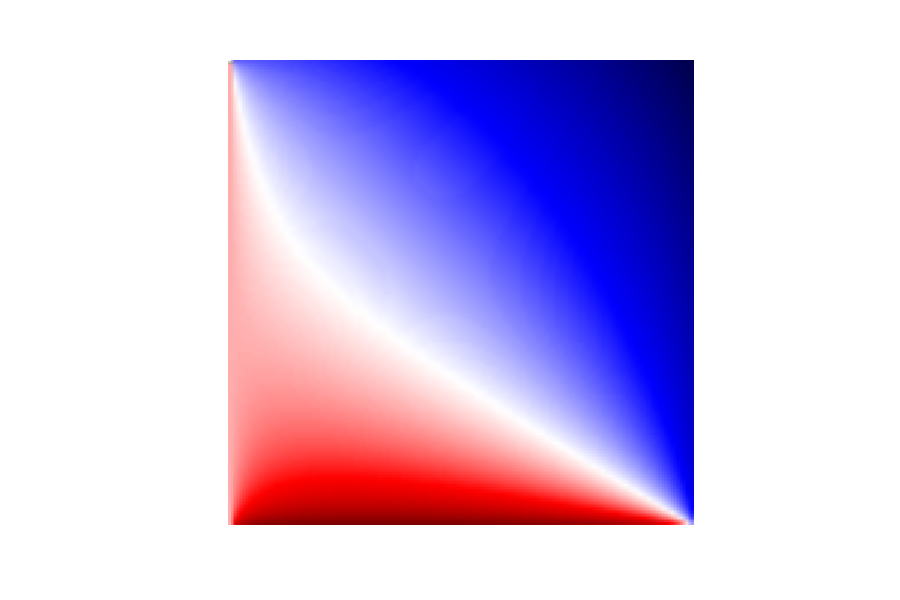
\includegraphics[width = 0.7\textwidth]{../img/WSLS-Analytical}}
\caption{A comparison of a fingerprint plot from previous literature to asses the suitability of the Seismic colour map}
\label{fig:WSLS-ashlock-comparison}
\end{figure}

With the knowledge that the choice of colourmap is appropriate, a comparison can now be made between analytical fingerprints and numerical ones obtained via the Axelrod-Python library.
Table \ref{tab:fingerprint-functions} gives the exact fingerprint functions of several well known strategies that will then be used to validate the numerical versions.

\begin{table}[htbp]
\centering
\renewcommand{\arraystretch}{2}
\setlength{\tabcolsep}{12pt}
\begin{tabular}{l l}
\toprule
Strategy & Analytical Fingerprint Function\\
\midrule
TitForTat &  $\displaystyle \frac{y^2 + 5xy + 3x^2}{(x + y)^2} $\\
Psycho (Anti TitForTat& $\displaystyle \frac{4(y-1)(x-1) + 5(y-1)^2}{2(y-1)(x-1) + (x-1)^2 + (y-1)^2} $ \\
WinStayLoseShit (Pavlov) & $\displaystyle \frac{(3x+y)(x-1) + 5y(y-1)}{(x+2y)(x-1) + y(y-1)} $\\
AllC (Cooperator) & $\displaystyle 3 - 3y $ \\
AllD (Defector) & $\displaystyle 4x + 1 $\\
\bottomrule
\end{tabular}
\caption{A selection of exact fingerprint functions for well known strategies. The probe used is TitForTat.}
\label{tab:fingerprint-functions}
\end{table}

Figures \ref{fig:TFT-comparison} \ref{fig:Psycho-comparison} \ref{fig:WSLS-comparison} \ref{fig:Cooperator-comparison} \ref{fig:Defector-comparison} compare plots of known exact fingerprint functions with analytical approximations obtained with the Axelrod-Python library.
The analytical plots were created with the code seen in listing \ref{lst:create-several-fingerprints}.
The parameters \mintinline{python}{turns=500, repetitions=200, step=0.01} are as described in section \ref{sec:fingerprint-implementation}.
The parameter \mintinline{python}{processes=0} ensures that the function will use the maximum number of cores available on the computer.

\begin{listing}[hbtp!]
\begin{ExampleCode}
import axelrod as axl
strats = [axl.TitForTat, axl.WinStayLoseShift, axl.AntiTitForTat,
          axl.Cooperator, axl.Defector]
for s in strats:
    probe = axl.TitForTat
    af = axl.AshlockFingerprint(s, probe)
    data = af.fingerprint(turns=500, repetitions=200, step=0.01, processes=0)
    p = af.plot()
    p.savefig('{}-Numerical.pdf'.format(s.name))
\end{ExampleCode}
\caption{Code to create the numerical plots for several strategies}
\label{lst:create-several-fingerprints}
\end{listing}

\begin{figure}[htbp!]
\subfloat[Exact analytical fingerprint]{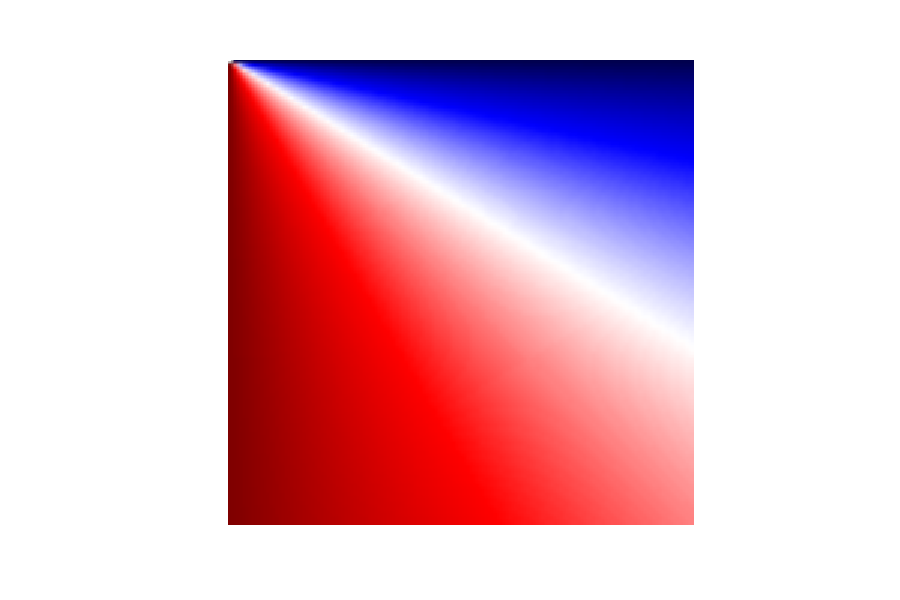
\includegraphics[width = 0.5\textwidth]{../img/TFT-Analytical.pdf}}
% \subfloat[Numerical Fingerprint]{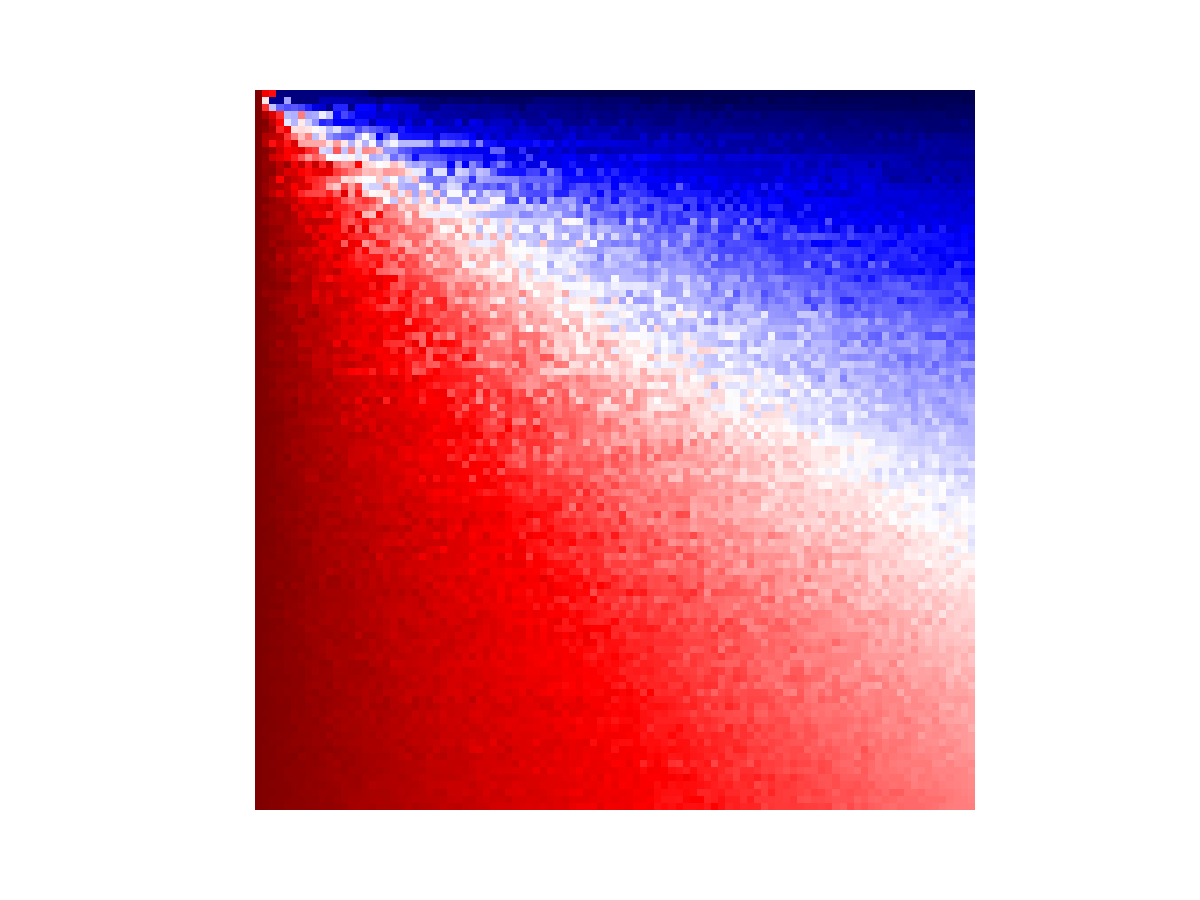
\includegraphics[width = 0.5\textwidth]{../img/Numerical/TitForTat.pdf}}
\caption{A comparison of the analytical fingerprint of TitForTat and the numerical version produced by Axelrod-Python library.}
\label{fig:TFT-comparison}
\end{figure}
\begin{figure}[htbp!]
\subfloat[Exact analytical fingerprint]{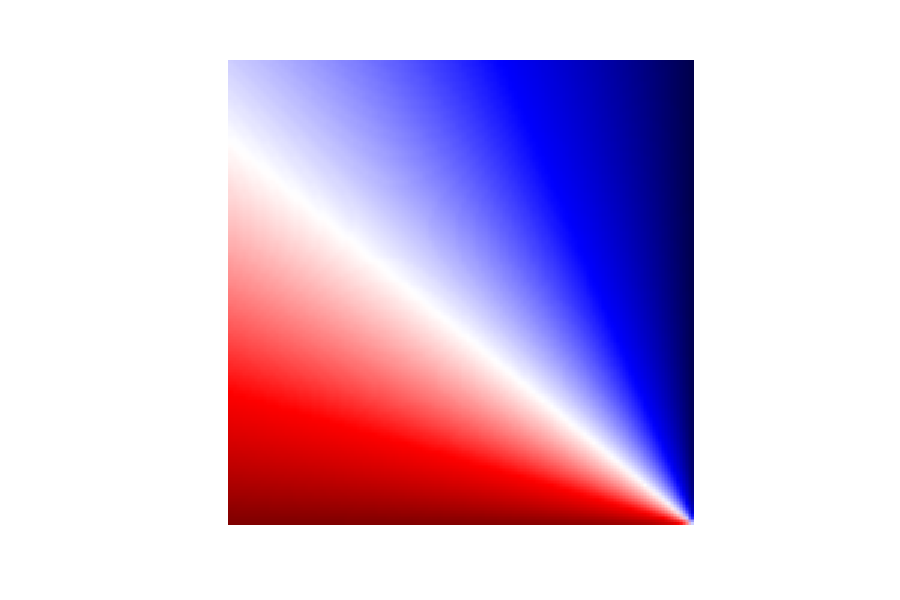
\includegraphics[width = 0.5\textwidth]{../img/Psycho-Analytical.pdf}}
% \subfloat[Numerical Fingerprint]{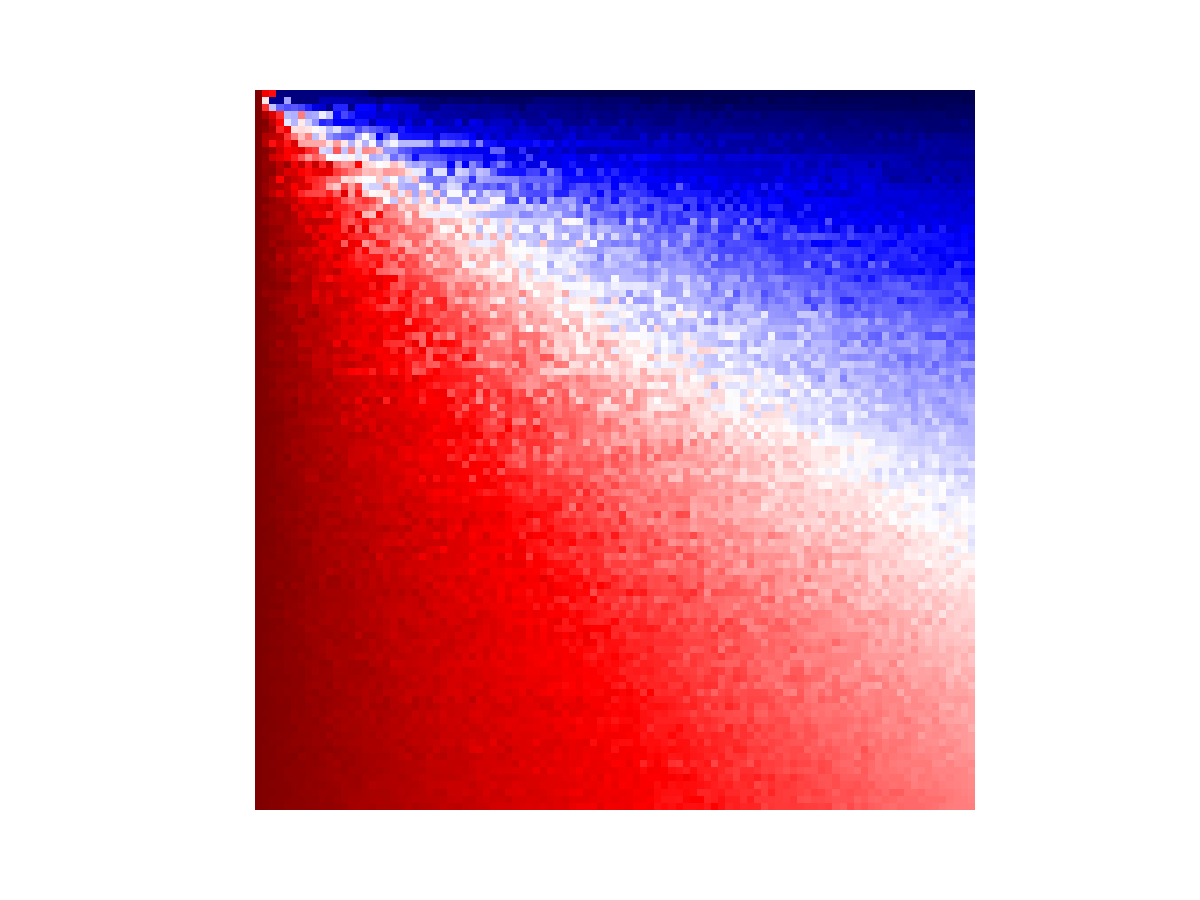
\includegraphics[width = 0.5\textwidth]{../img/Numerical/TitForTat.pdf}}
\caption{A comparison of the analytical fingerprint of Psycho and the numerical version produced by Axelrod-Python library.}
\label{fig:Psycho-comparison}
\end{figure}
\begin{figure}[htbp!]
\subfloat[Exact analytical fingerprint]{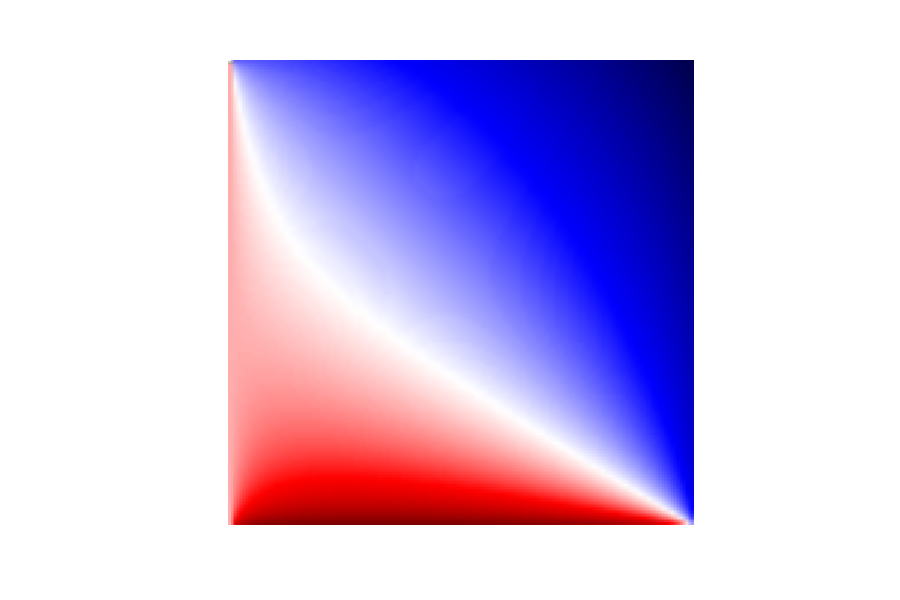
\includegraphics[width = 0.5\textwidth]{../img/WSLS-Analytical.pdf}}
% \subfloat[Numerical Fingerprint]{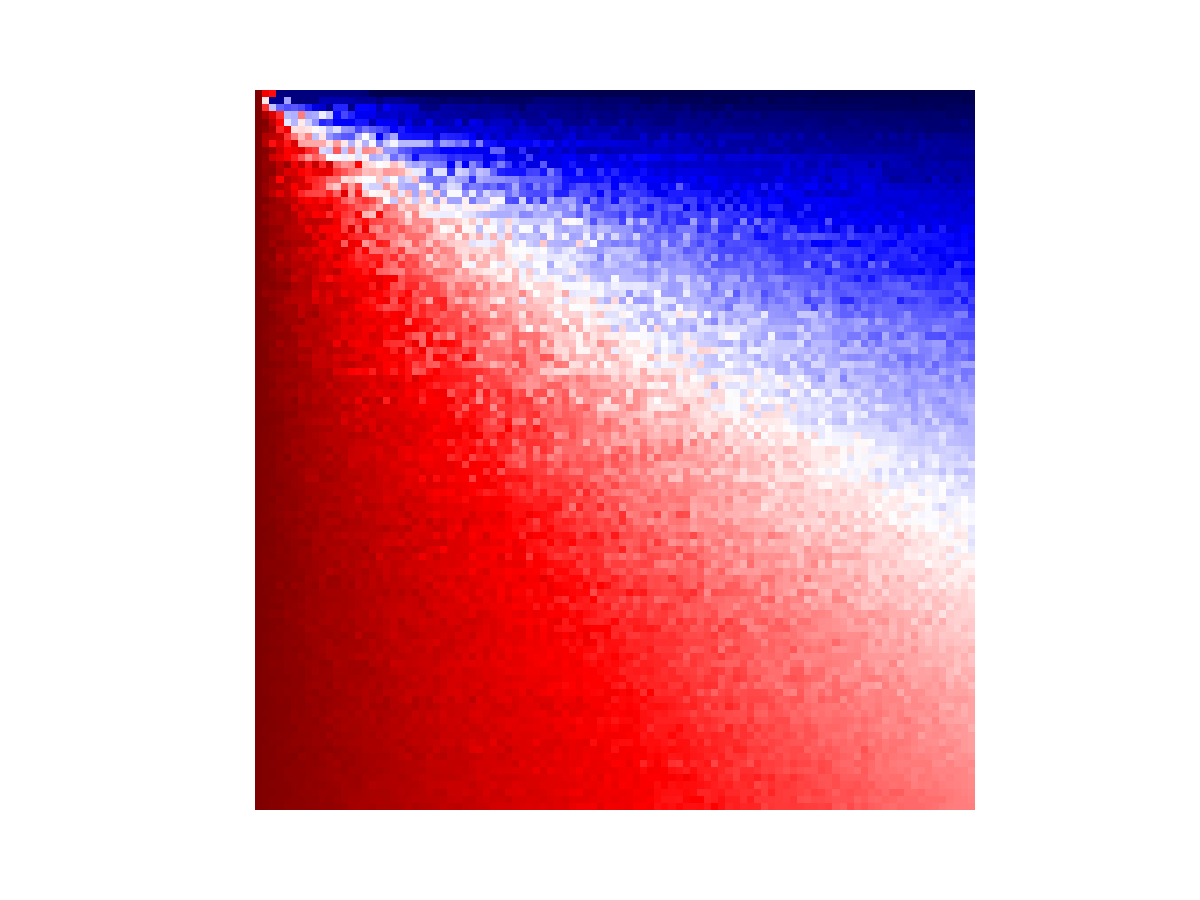
\includegraphics[width = 0.5\textwidth]{../img/Numerical/TitForTat.pdf}}
\caption{A comparison of the analytical fingerprint of WinStayLoseShit and the numerical version produced by Axelrod-Python library.}
\label{fig:WSLS-comparison}
\end{figure}
\begin{figure}[htbp!]
\subfloat[Exact analytical fingerprint]{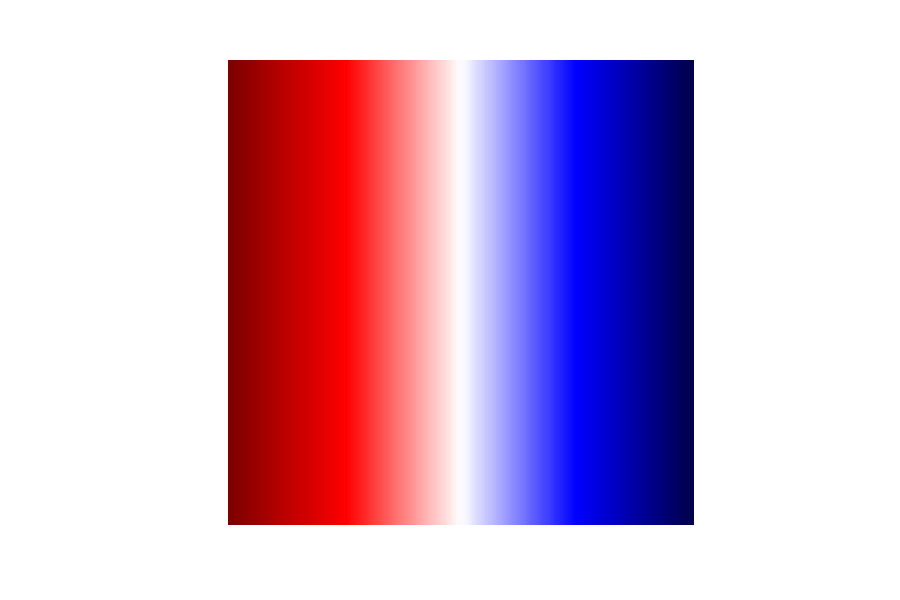
\includegraphics[width = 0.5\textwidth]{../img/AllC-Analytical.pdf}}
% \subfloat[Numerical Fingerprint]{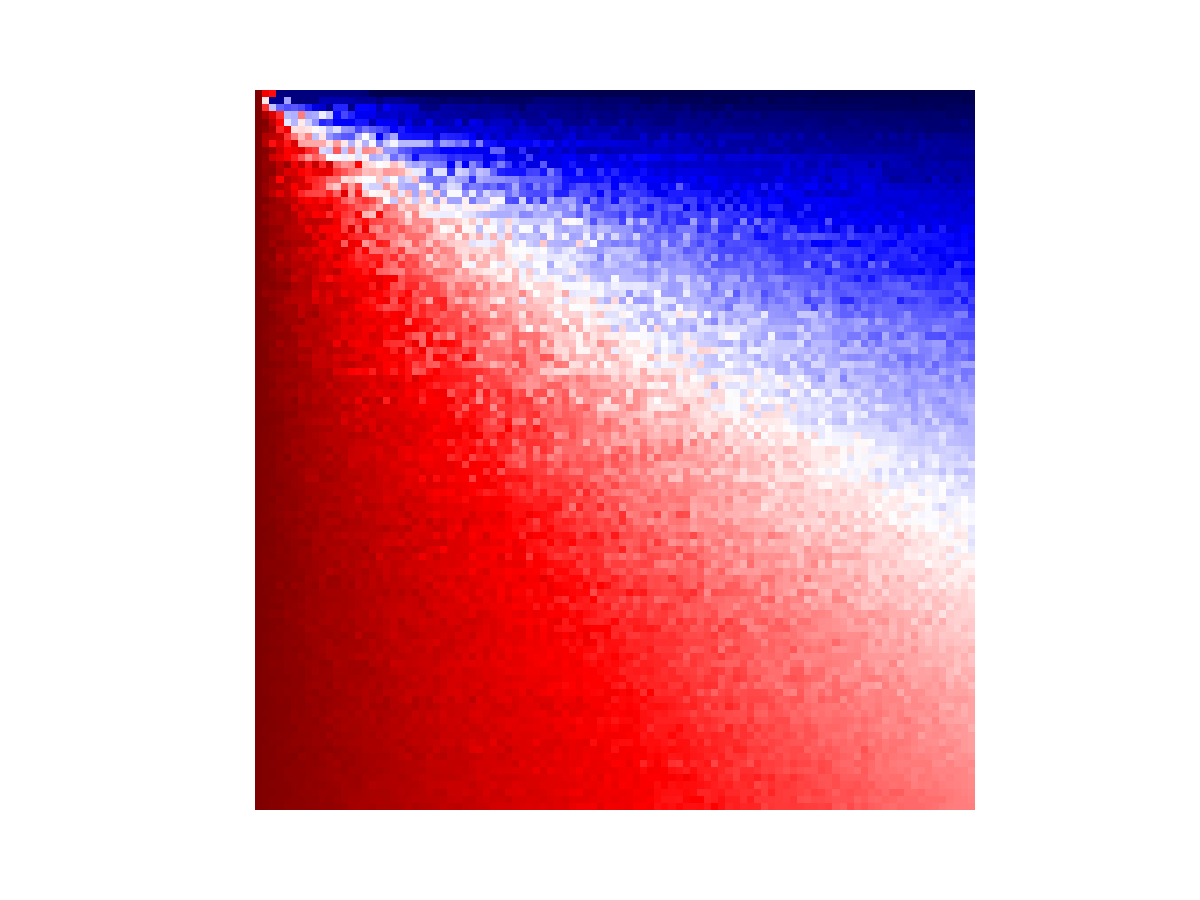
\includegraphics[width = 0.5\textwidth]{../img/Numerical/TitForTat.pdf}}
\caption{A comparison of the analytical fingerprint of Cooperator and the numerical version produced by Axelrod-Python library.}
\label{fig:Cooperator-comparison}
\end{figure}
\begin{figure}[htbp!]
\subfloat[Exact analytical fingerprint]{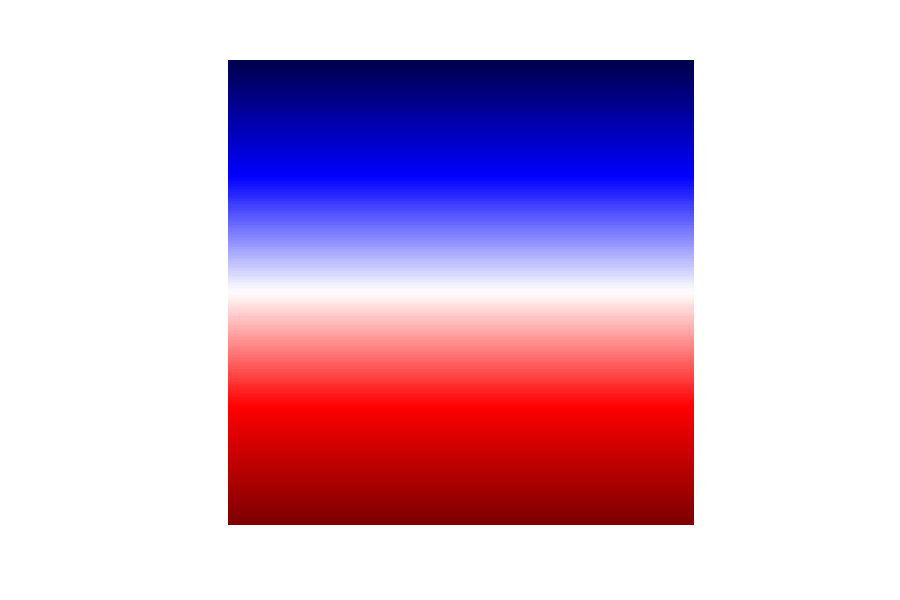
\includegraphics[width = 0.5\textwidth]{../img/AllD-Analytical.pdf}}
% \subfloat[Numerical Fingerprint]{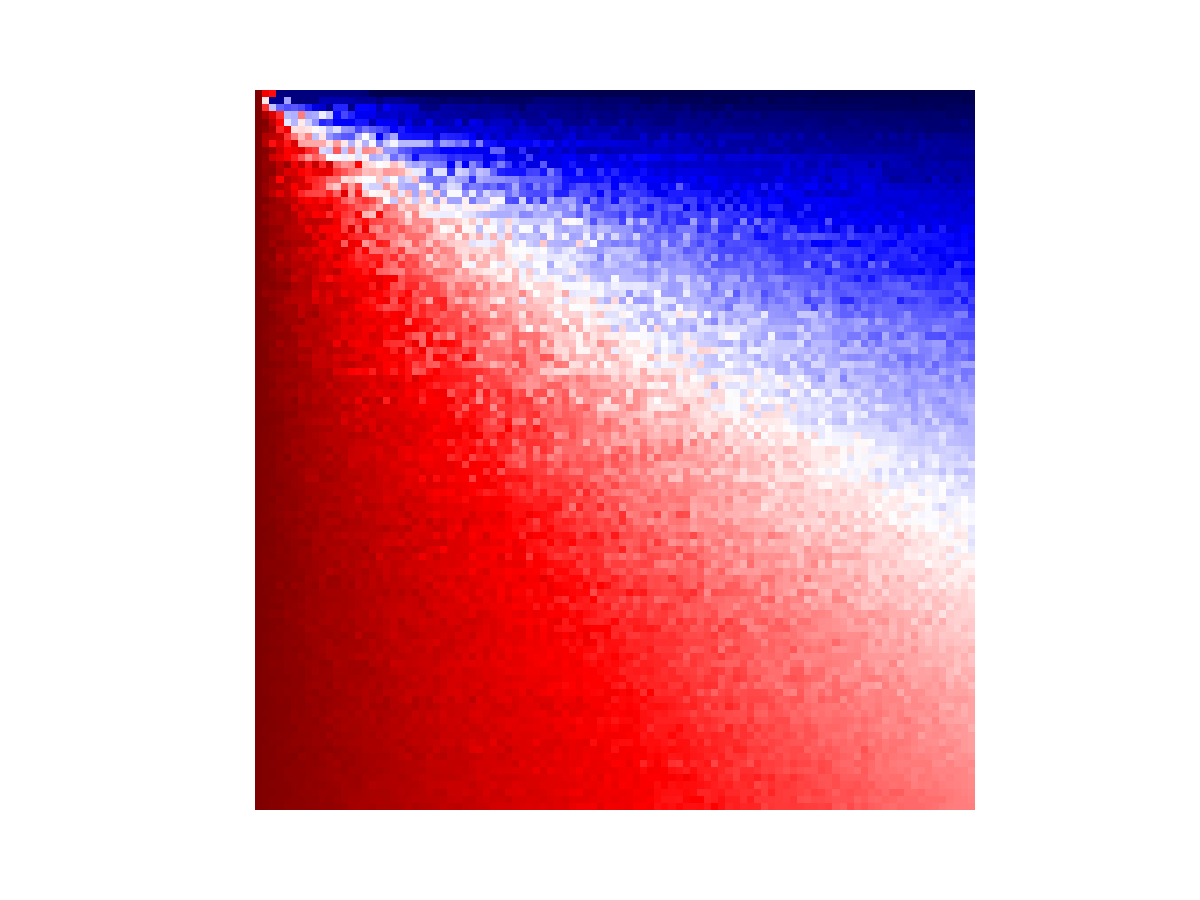
\includegraphics[width = 0.5\textwidth]{../img/Numerical/TitForTat.pdf}}
\caption{A comparison of the analytical fingerprint of Defector and the numerical version produced by Axelrod-Python library.}
\label{fig:Defector-comparison}
\end{figure}
